%%%%%%%%%%%%%%%%%%%%%%%%%%%%%%%%%%%%%%%%%%%%%%%%%%%%%%%%%%%%%%%%%%%%%%%%%%%%%%%%%%%%%%%%%%%%%%%%%%%%%%%%%%%%%%%%%%%%%%%%%%%%%%%%%%%%%%%%%%%%%%%%%%%%%%%%%%%%%%%%%%%
% Written By Michael Brodskiy
% Class: Fundamentals of Electronics
% Professor: M. Onabajo
%%%%%%%%%%%%%%%%%%%%%%%%%%%%%%%%%%%%%%%%%%%%%%%%%%%%%%%%%%%%%%%%%%%%%%%%%%%%%%%%%%%%%%%%%%%%%%%%%%%%%%%%%%%%%%%%%%%%%%%%%%%%%%%%%%%%%%%%%%%%%%%%%%%%%%%%%%%%%%%%%%%

\documentclass[12pt]{article} 
\usepackage{alphalph}
\usepackage[utf8]{inputenc}
\usepackage[russian,english]{babel}
\usepackage{titling}
\usepackage{amsmath}
\usepackage{graphicx}
\usepackage{enumitem}
\usepackage{amssymb}
\usepackage[super]{nth}
\usepackage{everysel}
\usepackage{ragged2e}
\usepackage{geometry}
\usepackage{multicol}
\usepackage{fancyhdr}
\usepackage{cancel}
\usepackage{siunitx}
\usepackage{physics}
\usepackage{tikz}
\usepackage{mathdots}
\usepackage{yhmath}
\usepackage{cancel}
\usepackage{color}
\usepackage{array}
\usepackage{multirow}
\usepackage{gensymb}
\usepackage{tabularx}
\usepackage{extarrows}
\usepackage{booktabs}
\usepackage{lastpage}
\usetikzlibrary{fadings}
\usetikzlibrary{patterns}
\usetikzlibrary{shadows.blur}
\usetikzlibrary{shapes}

\geometry{top=1.0in,bottom=1.0in,left=1.0in,right=1.0in}
\newcommand{\subtitle}[1]{%
  \posttitle{%
    \par\end{center}
    \begin{center}\large#1\end{center}
    \vskip0.5em}%

}
\usepackage{hyperref}
\hypersetup{
colorlinks=true,
linkcolor=blue,
filecolor=magenta,      
urlcolor=blue,
citecolor=blue,
}


\title{Homework 4}
\date{\today}
\author{Michael Brodskiy\\ \small Professor: M. Onabajo}

\begin{document}

\maketitle

\begin{enumerate}

  \item

    \begin{enumerate}

      \item 

        Let us assume the diode is in forward bias. In this case, the circuit consists simply of the source and resistor, which gives us current:

        $$I=\frac{v_{in}}{R}$$

        Given that this value is  sinusoidal, when greater than zero, we know that our initial assumption was true. When the voltage is zero or negative, the ideal diode is reverse-biased. We can now proceed to say:

        $$v_o=\left\{\begin{array}{ll} v_{in}, & v_{in}>0\\ 0, & v_{in}\leq 0\end{array}$$

          Given that the given equation is:

          $$v_{in}=10\sin(200\pi t)$$

          we know that $v_{in}$ is positive when $2n\pi\leq 200\pi t\leq (2n+1)\pi$, with $n=0,1,2\cdots$. This gives: $(n/100)\leq t\leq (2n+1)/200$, which we can use to plot the transfer function ($v_o/v_{in}$):

          $$H(t)=\frac{v_o}{v_{in}}=\left\{\begin{array}{ll} 1, & (n/100)\leq t\leq (2n+1)/200\\ 0, & \text{otherwise}\end{array}$$

            \begin{figure}[H]
              \centering
              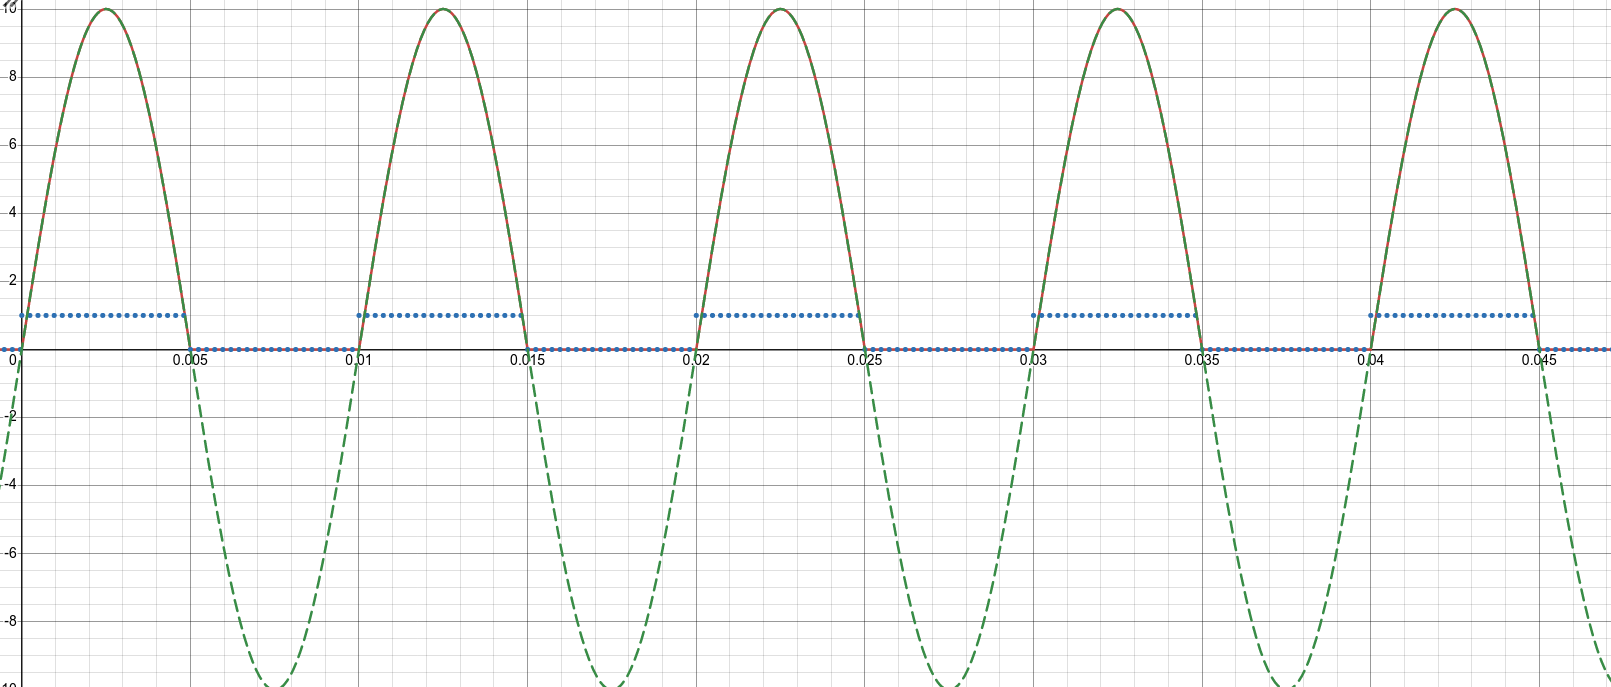
\includegraphics[width=.9\textwidth]{Figures/HW4-1a}
              \caption{$H(t)$ (\textcolor{blue}{blue}), $v_{in}$ (\textcolor{green}{green}), and $v_{o}$ (\textcolor{red}{red}) in Time Domain}
              \label{fig:1}
            \end{figure}

            Plotting $v_o$ versus $v_{in}$, we find a linear relationship:

            \begin{figure}[H]
              \centering
              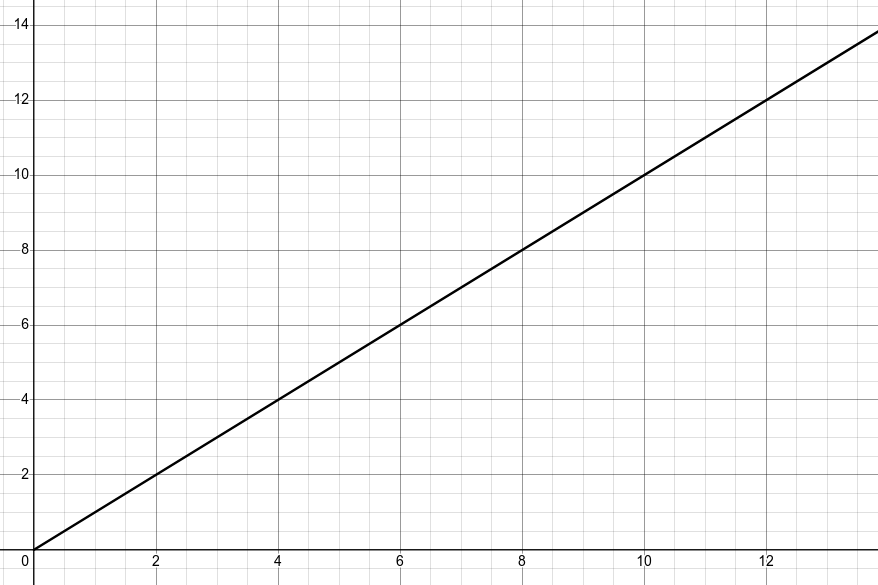
\includegraphics[width=.9\textwidth]{Figures/HW4-1a2}
              \caption{$v_o$ versus $v_{in}$ (1:1 relationship)}
              \label{fig:2}
            \end{figure}


      \item 

        Similar to part (a), let us assume this diode is forward biased. In this case, we have the same current flow, indicating that this assumption is correct; however, the cycle is reversed in that $v_o$ is zero when the diode is forward-biased, and $v_o=v_{in}$ when it is reverse biased. Thus, we may write this as:

        $$v_o=\left\{\begin{array}{ll} v_{in}, & v_{in}\leq0\\ 0, & v_{in}>0\end{array}$$
        $$H(t)=\frac{v_o}{v_{in}}=\left\{\begin{array}{ll} 0, & (n/100)\leq t\leq (2n+1)/200\\ 1, & \text{otherwise}\end{array}$$

          This gives us the following plot:

            \begin{figure}[H]
              \centering
              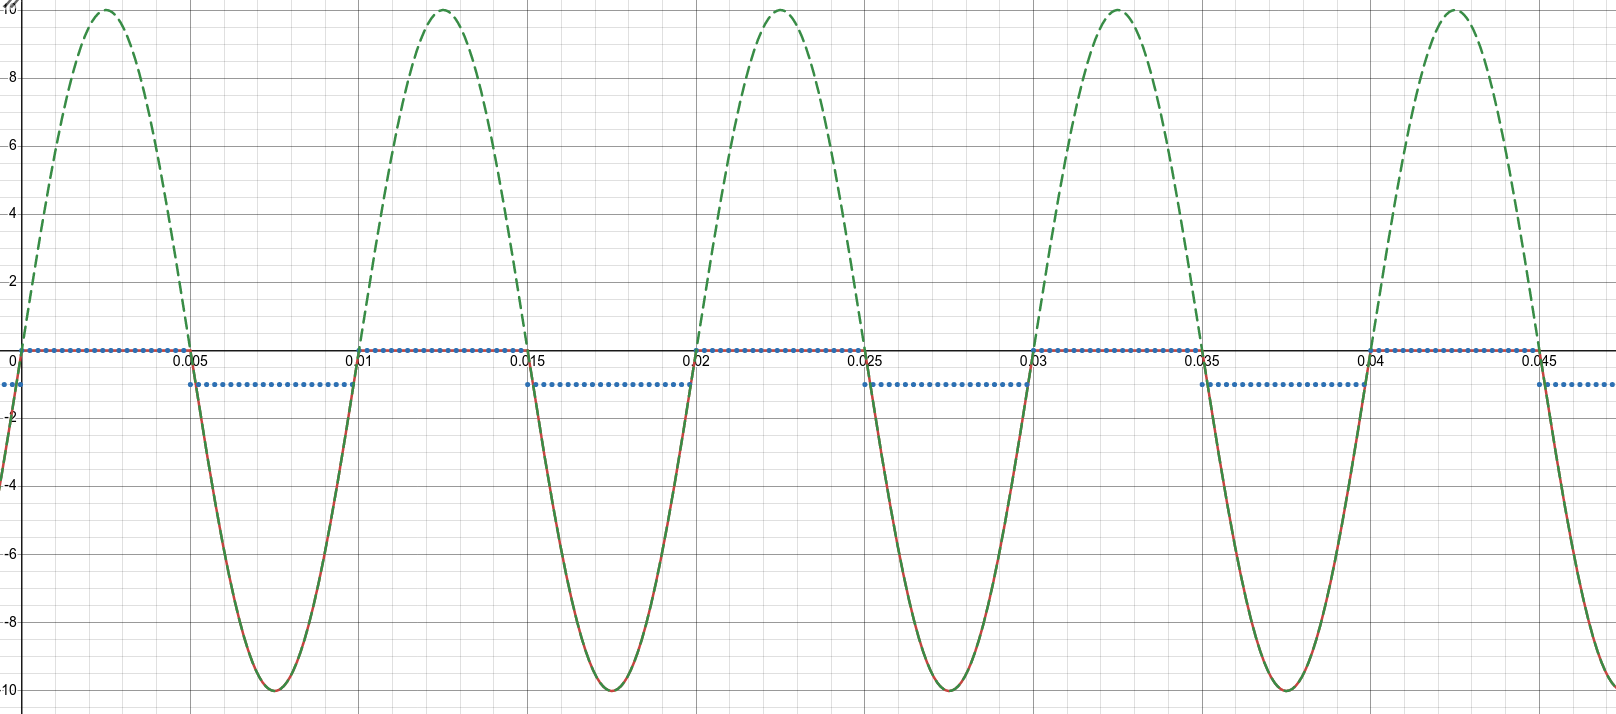
\includegraphics[width=.9\textwidth]{Figures/HW4-1b}
              \caption{$H(t)$ (\textcolor{blue}{blue}), $v_{in}$ (\textcolor{green}{green}), and $v_{o}$ (\textcolor{red}{red}) in Time Domain}
              \label{fig:4}
            \end{figure}

            Plotting $v_o$ versus $v_{in}$, we find a linear relationship:

            \begin{figure}[H]
              \centering
              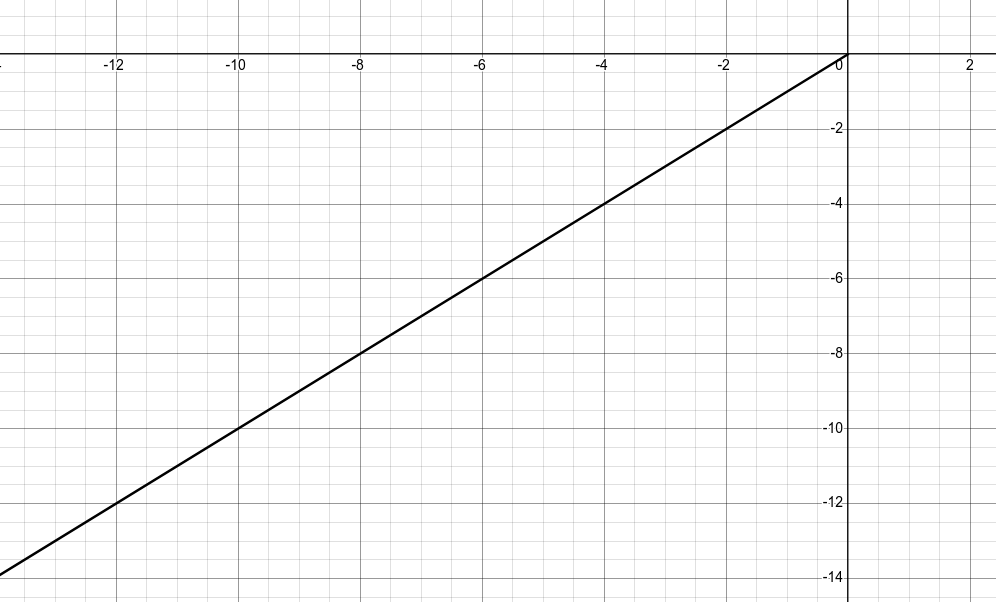
\includegraphics[width=.9\textwidth]{Figures/HW4-1b2}
              \caption{$v_o$ versus $v_{in}$ (1:-1 relationship)}
              \label{fig:4}
            \end{figure}

      \item 

        Using a non-ideal, constant voltage drop (CVD) model, we know that, since there is one diode in each circuit, the output will be $.7[\si{\volt}]$ less for a forward-biased diode. For circuit 1, this gives us:

            \begin{figure}[H]
              \centering
              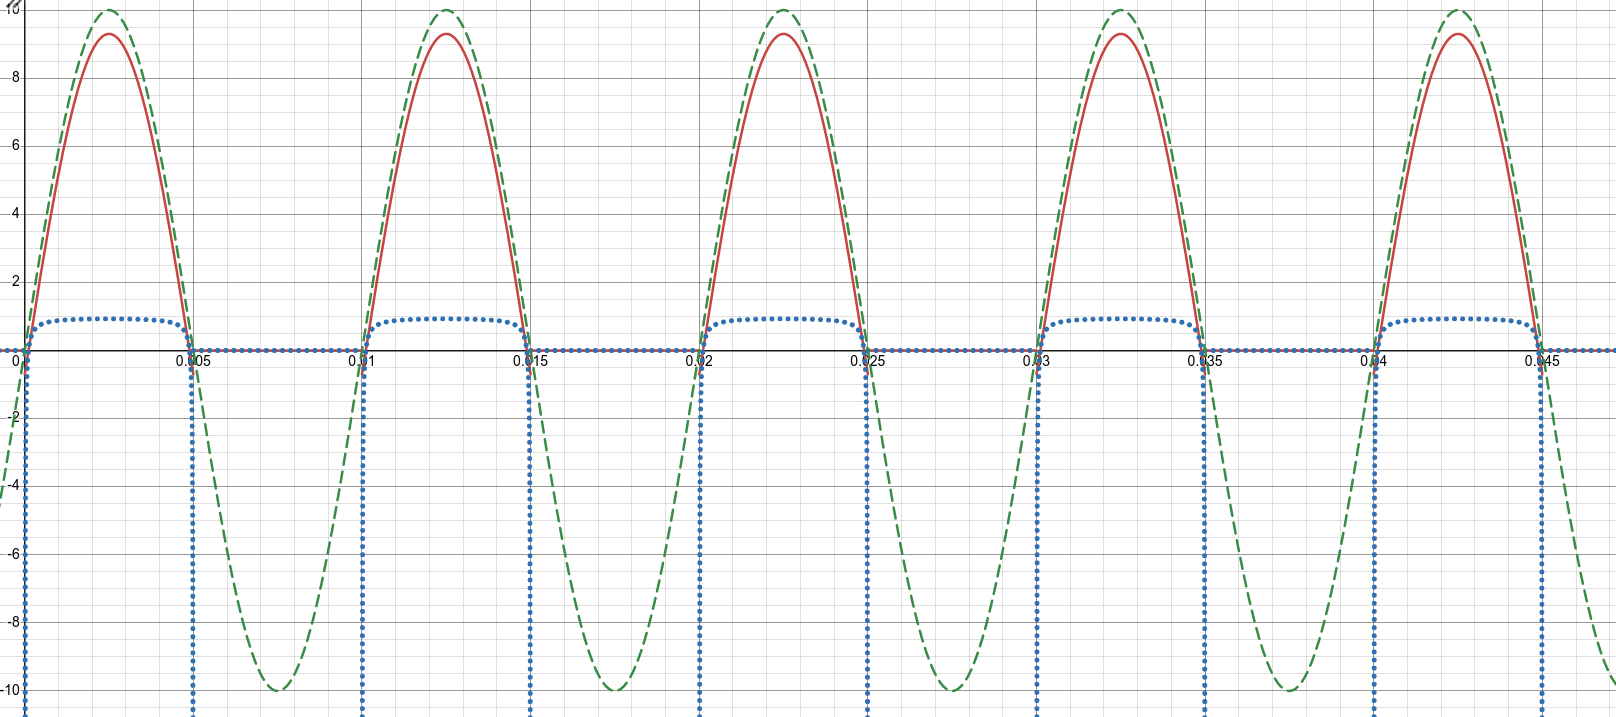
\includegraphics[width=.9\textwidth]{Figures/HW4-1c}
              \caption{$H(t)$ (\textcolor{blue}{blue}), $v_{in}$ (\textcolor{green}{green}), and $v_{o}$ (\textcolor{red}{red}) in Time Domain}
              \label{fig:5}
            \end{figure}

            \begin{figure}[H]
              \centering
              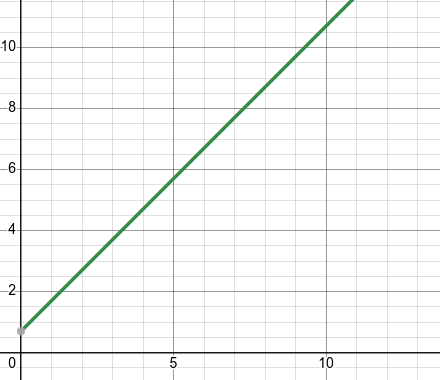
\includegraphics[width=.7\textwidth]{Figures/HW4-1c2}
              \caption{$v_o$ versus $v_{in}$}
              \label{fig:6}
            \end{figure}

            Since the voltage was, initially, just zero when the diode was forward-biased (in the ideal case), with CVD we get:

            \begin{figure}[H]
              \centering
              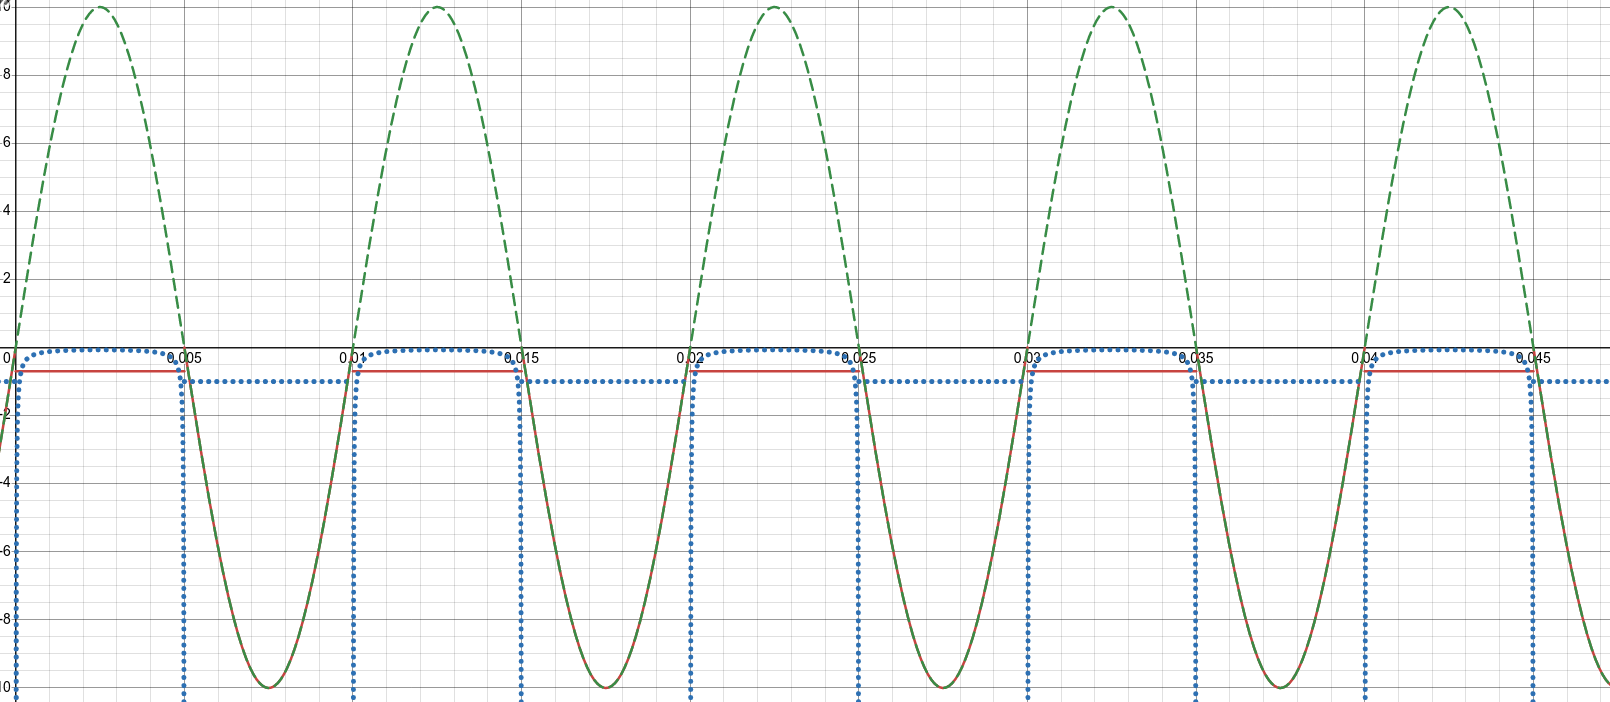
\includegraphics[width=.9\textwidth]{Figures/HW4-1c3}
              \caption{$H(t)$ (\textcolor{blue}{blue}), $v_{in}$ (\textcolor{green}{green}), and $v_{o}$ (\textcolor{red}{red}) in Time Domain}
              \label{fig:7}
            \end{figure}

            \begin{figure}[H]
              \centering
              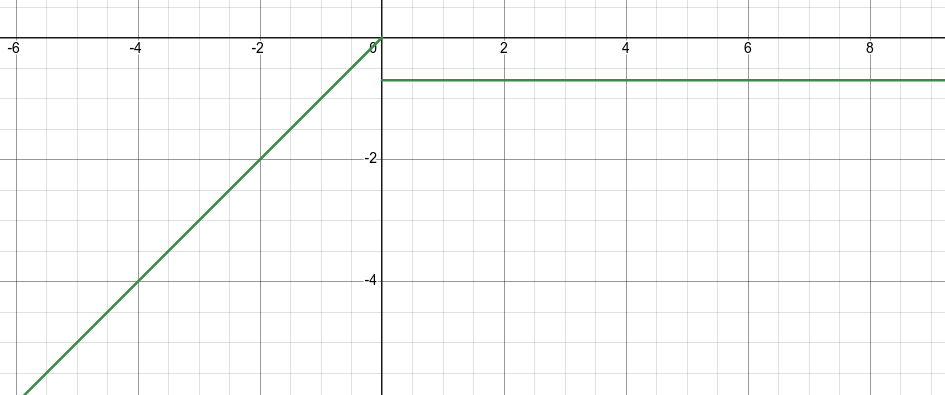
\includegraphics[width=.9\textwidth]{Figures/HW4-1c4}
              \caption{$H(t)$ (\textcolor{blue}{blue}), $v_{in}$ (\textcolor{green}{green}), and $v_{o}$ (\textcolor{red}{red}) in Time Domain}
              \label{fig:8}
            \end{figure}

    \end{enumerate}

  \item

    \begin{enumerate}

      \item We begin by finding the maximum voltage value of the rectifier. Since we know the peak-to-peak ripple, we find the extrema:

        $$V_{ext}=V_{avg}\pm\frac{V_{pp}}{2}$$
        $$V_{ext}=9\pm 1$$

        Thus, we see the minimum load voltage is $8[\si{\volt}]$, with:

        $$\boxed{V_{max}=10[\si{\volt}]}$$

      \item 

        We know that the peak secondary voltage must be $10[\si{\volt}]$. Given this, we can write the turns ratio as (note we need to convert to RMS value):

        $$n=\frac{N_1}{N_2}=\frac{V_1}{V_2}$$
        $$n=\frac{220}{10\sqrt{2}}$$
        $$\boxed{n=15.6}$$

      \item 

        We can write the equation for capacitance as:

        $$C=\frac{I_LT}{V_r}$$
        $$C=\frac{(.1)(.01667)}{2}$$
        $$\boxed{C=.833[\si{\milli\farad}]}$$

        We can now construct the circuit and get:
        
        \begin{figure}[H]
          \centering
          \tikzset{every picture/.style={line width=0.75pt}} %set default line width to 0.75pt        

\begin{tikzpicture}[x=0.75pt,y=0.75pt,yscale=-1,xscale=1]
%uncomment if require: \path (0,863); %set diagram left start at 0, and has height of 863

%Shape: Circle [id:dp13333077766246426] 
\draw   (122,188.5) .. controls (122,174.97) and (132.97,164) .. (146.5,164) .. controls (160.03,164) and (171,174.97) .. (171,188.5) .. controls (171,202.03) and (160.03,213) .. (146.5,213) .. controls (132.97,213) and (122,202.03) .. (122,188.5) -- cycle ;
%Curve Lines [id:da44603915985021503] 
\draw    (129,190) .. controls (145,174) and (149,206) .. (162,187) ;
%Straight Lines [id:da4414756688923631] 
\draw    (146.5,213) -- (146.5,265.42) ;
%Straight Lines [id:da7149052752569974] 
\draw    (146.5,111.58) -- (146.5,164) ;
%Straight Lines [id:da6721818443805452] 
\draw    (287.92,111.58) -- (146.5,111.58) ;
%Straight Lines [id:da8961401646328636] 
\draw    (287.92,265.42) -- (146.5,265.42) ;
%Shape: Inductor (Air Core) [id:dp5665935759216707] 
\draw   (287.92,111.58) -- (287.92,139.27) .. controls (298.43,139.67) and (307.41,143.51) .. (310.55,148.95) .. controls (313.7,154.39) and (310.35,160.32) .. (302.14,163.89) .. controls (295.73,166.63) and (287.44,167.75) .. (279.39,166.96) .. controls (276.25,166.96) and (273.71,165.58) .. (273.71,163.89) .. controls (273.71,162.19) and (276.25,160.81) .. (279.39,160.81) .. controls (287.44,160.02) and (295.73,161.14) .. (302.14,163.89) .. controls (308.97,167.08) and (312.84,171.53) .. (312.84,176.19) .. controls (312.84,180.85) and (308.97,185.3) .. (302.14,188.5) .. controls (295.73,191.25) and (287.44,192.37) .. (279.39,191.58) .. controls (276.25,191.58) and (273.71,190.2) .. (273.71,188.5) .. controls (273.71,186.8) and (276.25,185.42) .. (279.39,185.42) .. controls (287.44,184.63) and (295.73,185.75) .. (302.14,188.5) .. controls (308.97,191.7) and (312.84,196.15) .. (312.84,200.81) .. controls (312.84,205.47) and (308.97,209.92) .. (302.14,213.11) .. controls (295.73,215.86) and (287.44,216.98) .. (279.39,216.19) .. controls (276.25,216.19) and (273.71,214.81) .. (273.71,213.11) .. controls (273.71,211.42) and (276.25,210.04) .. (279.39,210.04) .. controls (287.44,209.25) and (295.73,210.37) .. (302.14,213.11) .. controls (310.35,216.68) and (313.7,222.61) .. (310.55,228.05) .. controls (307.41,233.49) and (298.43,237.33) .. (287.92,237.73) -- (287.92,265.42) ;
%Shape: Inductor (Air Core) [id:dp3974548882688711] 
\draw   (337.75,265.42) -- (337.75,237.73) .. controls (327.24,237.33) and (318.26,233.49) .. (315.12,228.05) .. controls (311.98,222.61) and (315.32,216.68) .. (323.54,213.11) .. controls (329.95,210.37) and (338.23,209.25) .. (346.28,210.04) .. controls (349.42,210.04) and (351.97,211.42) .. (351.97,213.11) .. controls (351.97,214.81) and (349.42,216.19) .. (346.28,216.19) .. controls (338.23,216.98) and (329.95,215.86) .. (323.54,213.11) .. controls (316.71,209.92) and (312.84,205.47) .. (312.84,200.81) .. controls (312.84,196.15) and (316.71,191.7) .. (323.54,188.5) .. controls (329.95,185.75) and (338.23,184.63) .. (346.28,185.42) .. controls (349.42,185.42) and (351.97,186.8) .. (351.97,188.5) .. controls (351.97,190.2) and (349.42,191.58) .. (346.28,191.58) .. controls (338.23,192.37) and (329.95,191.25) .. (323.54,188.5) .. controls (316.71,185.3) and (312.84,180.85) .. (312.84,176.19) .. controls (312.84,171.53) and (316.71,167.08) .. (323.54,163.89) .. controls (329.95,161.14) and (338.23,160.02) .. (346.28,160.81) .. controls (349.42,160.81) and (351.97,162.19) .. (351.97,163.89) .. controls (351.97,165.58) and (349.42,166.96) .. (346.28,166.96) .. controls (338.23,167.75) and (329.95,166.63) .. (323.54,163.89) .. controls (315.32,160.32) and (311.98,154.39) .. (315.12,148.95) .. controls (318.26,143.51) and (327.24,139.67) .. (337.75,139.27) -- (337.75,111.58) ;
%Straight Lines [id:da9771108245872508] 
\draw    (479.17,265.42) -- (337.75,265.42) ;
%Shape: Diode [id:dp37794795991982333] 
\draw   (380.18,94.08) -- (436.75,111.58) -- (380.18,129.08) -- (380.18,94.08) -- cycle (337.75,111.58) -- (380.18,111.58) (436.75,94.08) -- (436.75,129.08) (436.75,111.58) -- (479.17,111.58) ;
%Shape: Contact [id:dp3157159203292973] 
\draw   (479.17,164) -- (479.17,178.7) (479.17,213) -- (479.17,198.3) (497.59,178.7) -- (460.76,178.7) (497.59,198.3) -- (460.76,198.3) ;
%Straight Lines [id:da9006180717622023] 
\draw    (479.17,213) -- (479.17,265.42) ;
%Straight Lines [id:da29275782686803453] 
\draw    (479.17,111.58) -- (479.17,164) ;
%Straight Lines [id:da39570904222807435] 
\draw    (620.59,265.42) -- (479.17,265.42) ;
%Straight Lines [id:da8763639202981905] 
\draw    (620.59,111.58) -- (479.17,111.58) ;
%Shape: Circle [id:dp2091098875165296] 
\draw  [fill={rgb, 255:red, 0; green, 0; blue, 0 }  ,fill opacity=1 ] (615.59,265.42) .. controls (615.59,262.66) and (617.83,260.42) .. (620.59,260.42) .. controls (623.36,260.42) and (625.59,262.66) .. (625.59,265.42) .. controls (625.59,268.18) and (623.36,270.42) .. (620.59,270.42) .. controls (617.83,270.42) and (615.59,268.18) .. (615.59,265.42) -- cycle ;
%Shape: Circle [id:dp7795811126545164] 
\draw  [fill={rgb, 255:red, 0; green, 0; blue, 0 }  ,fill opacity=1 ] (615.59,111.58) .. controls (615.59,108.82) and (617.83,106.58) .. (620.59,106.58) .. controls (623.36,106.58) and (625.59,108.82) .. (625.59,111.58) .. controls (625.59,114.34) and (623.36,116.58) .. (620.59,116.58) .. controls (617.83,116.58) and (615.59,114.34) .. (615.59,111.58) -- cycle ;
%Straight Lines [id:da2478405062160971] 
\draw    (479.17,99.58) -- (618.59,99.58) ;
\draw [shift={(620.59,99.58)}, rotate = 180] [color={rgb, 255:red, 0; green, 0; blue, 0 }  ][line width=0.75]    (10.93,-3.29) .. controls (6.95,-1.4) and (3.31,-0.3) .. (0,0) .. controls (3.31,0.3) and (6.95,1.4) .. (10.93,3.29)   ;

% Text Node
\draw (173,188.5) node [anchor=west] [inner sep=0.75pt]    {$V_{s}$};
% Text Node
\draw (144.5,137.79) node [anchor=east] [inner sep=0.75pt]    {$+$};
% Text Node
\draw (144.5,239.21) node [anchor=east] [inner sep=0.75pt]    {$-$};
% Text Node
\draw (276.92,108.18) node [anchor=south west] [inner sep=0.75pt]    {$n=15.56$};
% Text Node
\draw (499.59,201.7) node [anchor=north west][inner sep=0.75pt]    {$.833\left[\text{mF}\right]$};
% Text Node
\draw (620.59,198) node [anchor=south] [inner sep=0.75pt]   [align=left] {Load};
% Text Node
\draw (549.88,96.18) node [anchor=south] [inner sep=0.75pt]    {$100\left[\text{mA}\right]$};


\end{tikzpicture}

          \caption{Half-Wave Rectifier Circuit, $V_{max}=10[\si{\volt}]$}
          \label{fig:9}
        \end{figure}

    \end{enumerate}

  \item

    \begin{enumerate}

      \item We can see that, if the diode is forward-biased, the current through $D$ can be found as (since the AC source can be omitted in the CVD model):

        $$I_D=\frac{7-.7}{5k}$$
        $$\boxed{I_D=1.26[\si{\milli\ampere}]}$$

        The output voltage is simply the drop across the diode, or:

        $$\boxed{V_D=.7[\si{\volt}]}$$

        Since the sinusoid can not exceed $-1[\si{\volt}]$, we see that the current is always positive, and, therefore, $D$ is always forward-biased.

      \item 

        We may write the Shockley equation as:

        $$I_D=I_S\left( e^{\frac{V_D}{nV_T}}-1 \right)$$

        Using the given values, we obtain:

        $$I_D=10^{-14}\left( e^{\frac{V_D}{(.025)}}-1 \right)$$

        Using $I_D$ from part (a), we get:

        $$(2\cdot10^{10})\left( 6.3 \right)+1=e^{40V_D}$$
        $$V_D=\ln[(2\cdot10^{10})\left( 6.3 \right)+1]$$
        $$\boxed{V_D=.639[\si{\volt}]}$$

      \item 

        The dynamic resistance formula may be written as:

        $$r_d=\frac{nV_T}{I_D}$$

        Which gets us:

        $$r_d=\frac{(.025)}{1.26\cdot10^{-3}}$$
        $$\boxed{r_d=19.841[\si{\ohm}]}$$

        This means that, in the small-signal model, the diode acts as a resistor, which means we have a voltage divider. We can find the AC voltage across the diode using:

        $$V_{ac}=(7-.7+V_s)\frac{19.841}{19.841+5000}$$
        $$V_{ac}=(.02445+.0039525\sin(120\pi t))$$

        This gets us:

        $$\boxed{V_{ac}=.02445+.0039525\sin(120\pi t)[\si{\volt}]}$$

        Summing the AC and DC components (the DC value would be from the CVD model), we get:

        $$\boxed{V_D=.72445+\left( 3.953\cdot 10^{-3} \right)\sin(120\pi t)[\si{\volt}]}$$

    \end{enumerate}

  \item We may begin by analyzing the circuit response to various values of $V_s$. Let us begin with the case when $V_s=0$. Here, $D_1$ would form an open circuit, which lets us calculate the current:

    $$I=\frac{5-.7}{6k}$$
    $$I=.7167[\si{\milli\ampere}]$$

    Thus, we can find $V_o$:

    $$V_o=5-5k(I)$$
    $$\boxed{V_o=1.4167[\si{\volt}]}$$

    Here, let us call the node above the single kilo-ohm resistor and ground as $V_n$. We know that, when $V_s-.7<V_x$, $D_1$ remains off, while $D_2$ is on, so the response remains the same as above (note: $V_x=.7167[\si{\volt}]$ when $D_1$ is off); however, let us test $V_s-.7\geq V_n$. In this case, $D_2$ is on until $V_n<4.3[\si{\volt}]$, or $V_s<5[\si{\volt}]$, at which point we can see:

    $$V_o=V_s$$

    In the case that $V_s\geq 5[\si{\volt}]$, $D_2$ shuts off, and the output is simply $5[\si{\volt}]$. Now that we have the pieces, we may plot the entire transfer function:

    \begin{figure}[H]
      \centering
      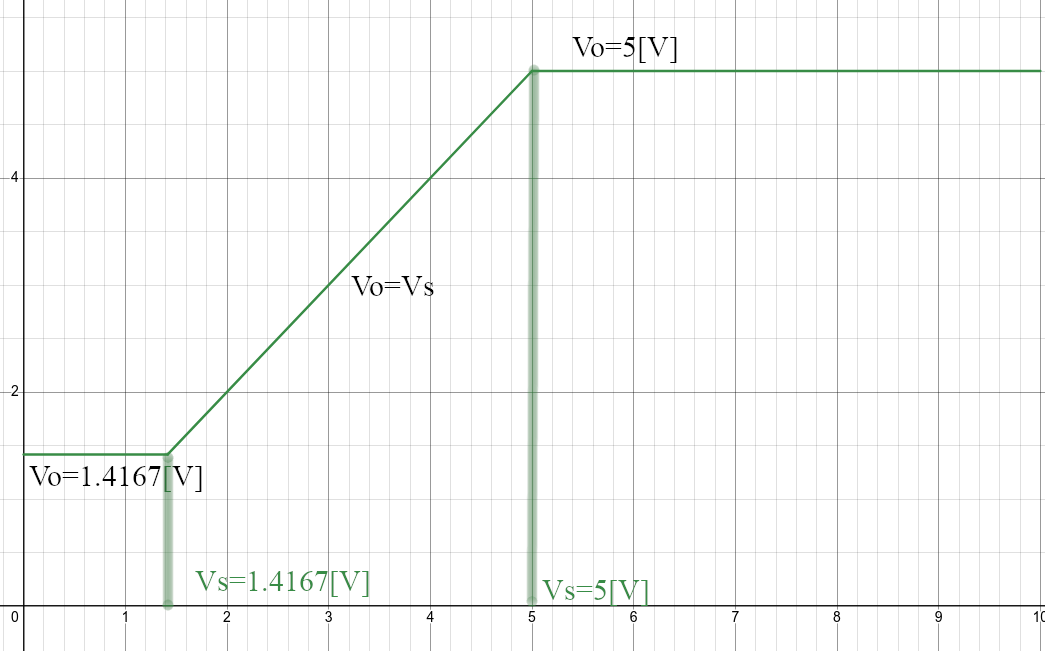
\includegraphics[width=.9\textwidth]{Figures/HW4-4}
      \caption{Transfer Characteristics of Given Circuit}
      \label{fig:10}
    \end{figure}

  \item We begin by generating the schematic:

    \begin{figure}[H]
      \centering
      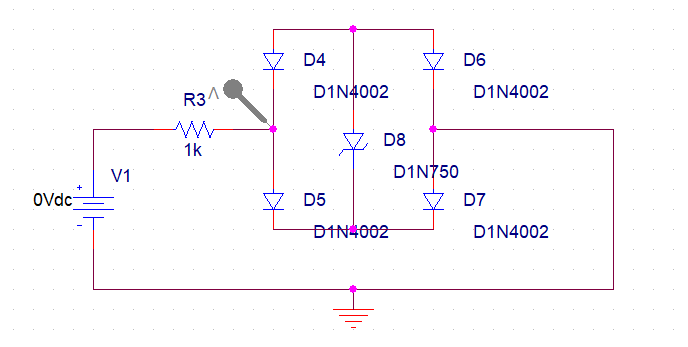
\includegraphics[width=.9\textwidth]{Figures/HW4-5}
      \caption{Schematic for DC Sweep}
      \label{fig:11}
    \end{figure}

    From here, we can simulate with the range $-15\leq V_{in}\leq 15$:

    \begin{figure}[H]
      \centering
      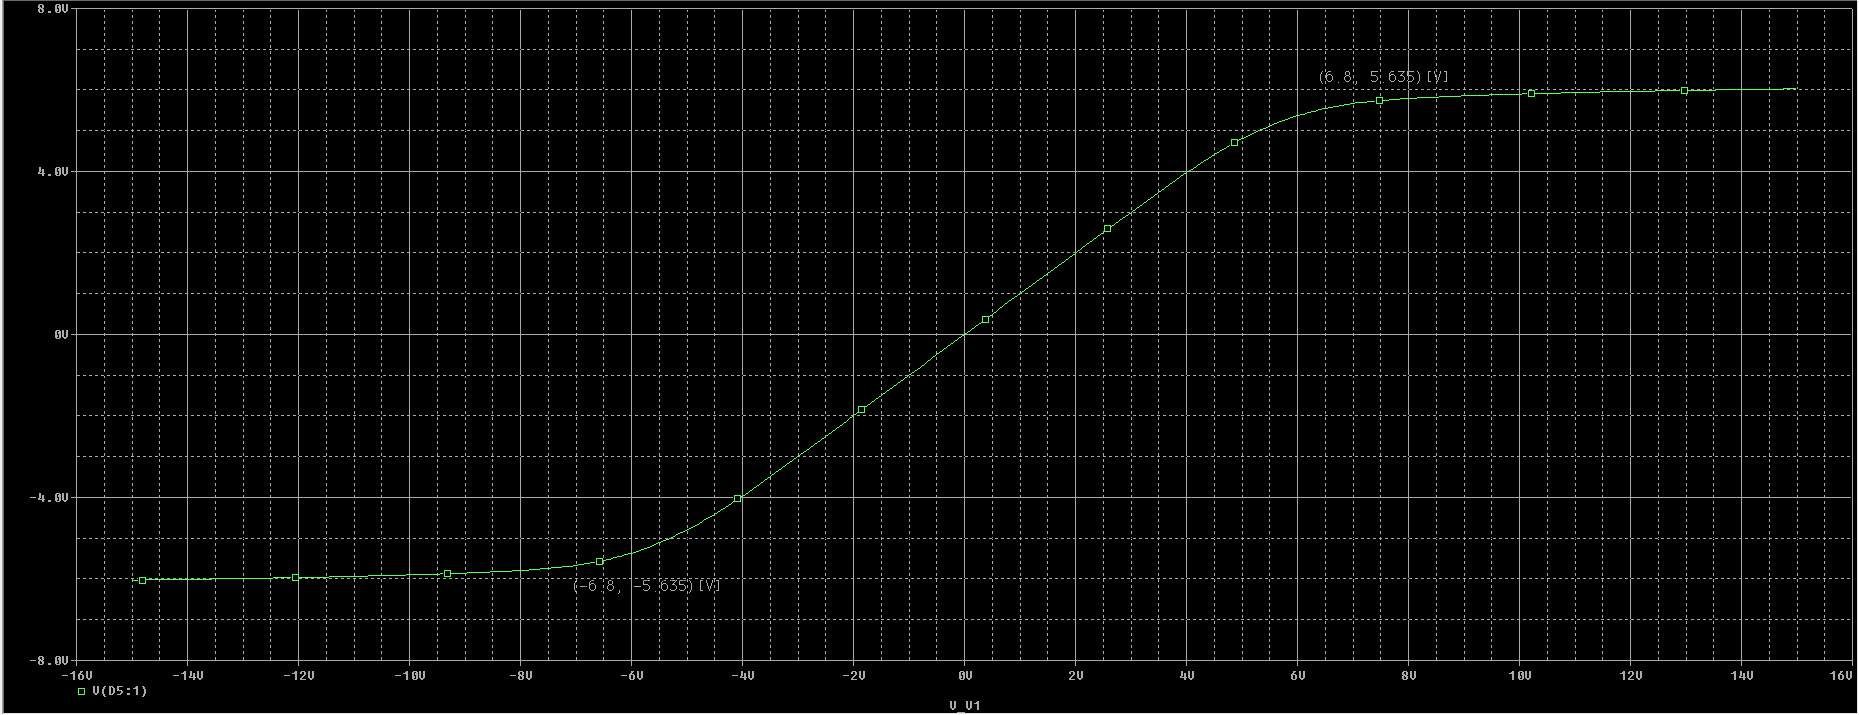
\includegraphics[width=.9\textwidth]{Figures/HW4-5b}
      \caption{DC Sweep Transfer Characteristics}
      \label{fig:12}
    \end{figure}

    With the sweep, we may see that the maximum voltage magnitude is approximately $6[\si{\volt}]$, as expected for the circuit. Furthermore, the knee values occur at, approximately, the voltage value of the zener diode, or $V_{z}=6.8[\si{\volt}]$. We can test the same circuit with an AC input:

    \begin{figure}[H]
      \centering
      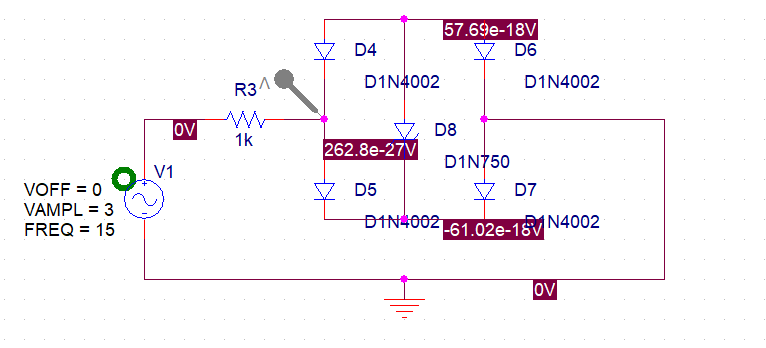
\includegraphics[width=.9\textwidth]{Figures/HW4-5c}
      \caption{Schematic for AC Sweep}
      \label{fig:13}
    \end{figure}

    Using this circuit, we obtain the results for a wave with magnitude $3[\si{\volt}]$ and $12[\si{\volt}]$:

    \begin{figure}[H]
      \centering
      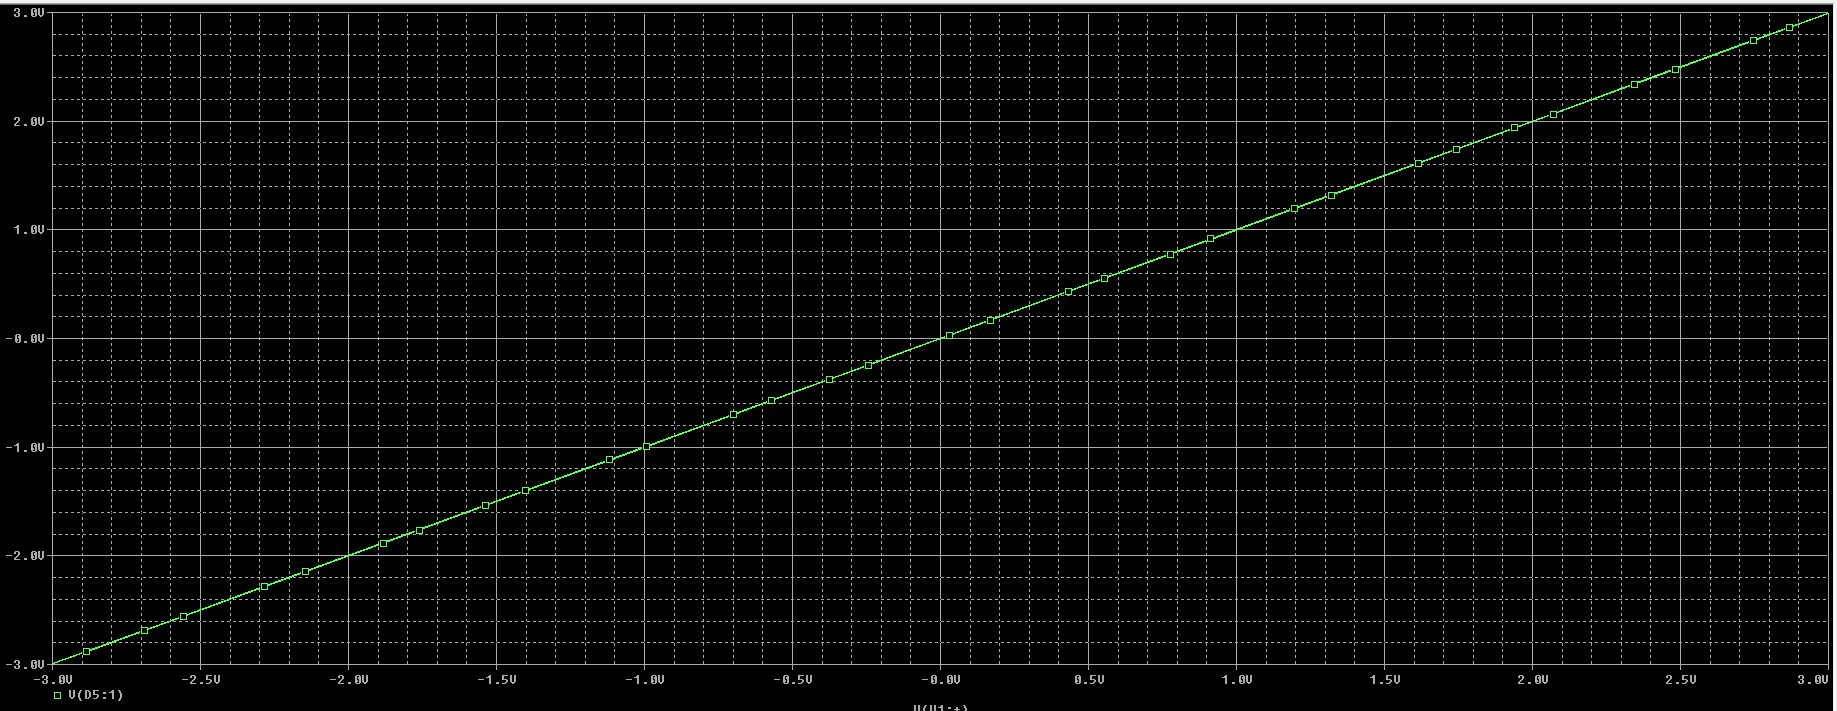
\includegraphics[width=.85\textwidth]{Figures/HW4-5d}
      \caption{Transfer Characteristics for $3[\si{\volt}]$ Amplitude Input}
      \label{fig:14}
    \end{figure}

    \begin{figure}[H]
      \centering
      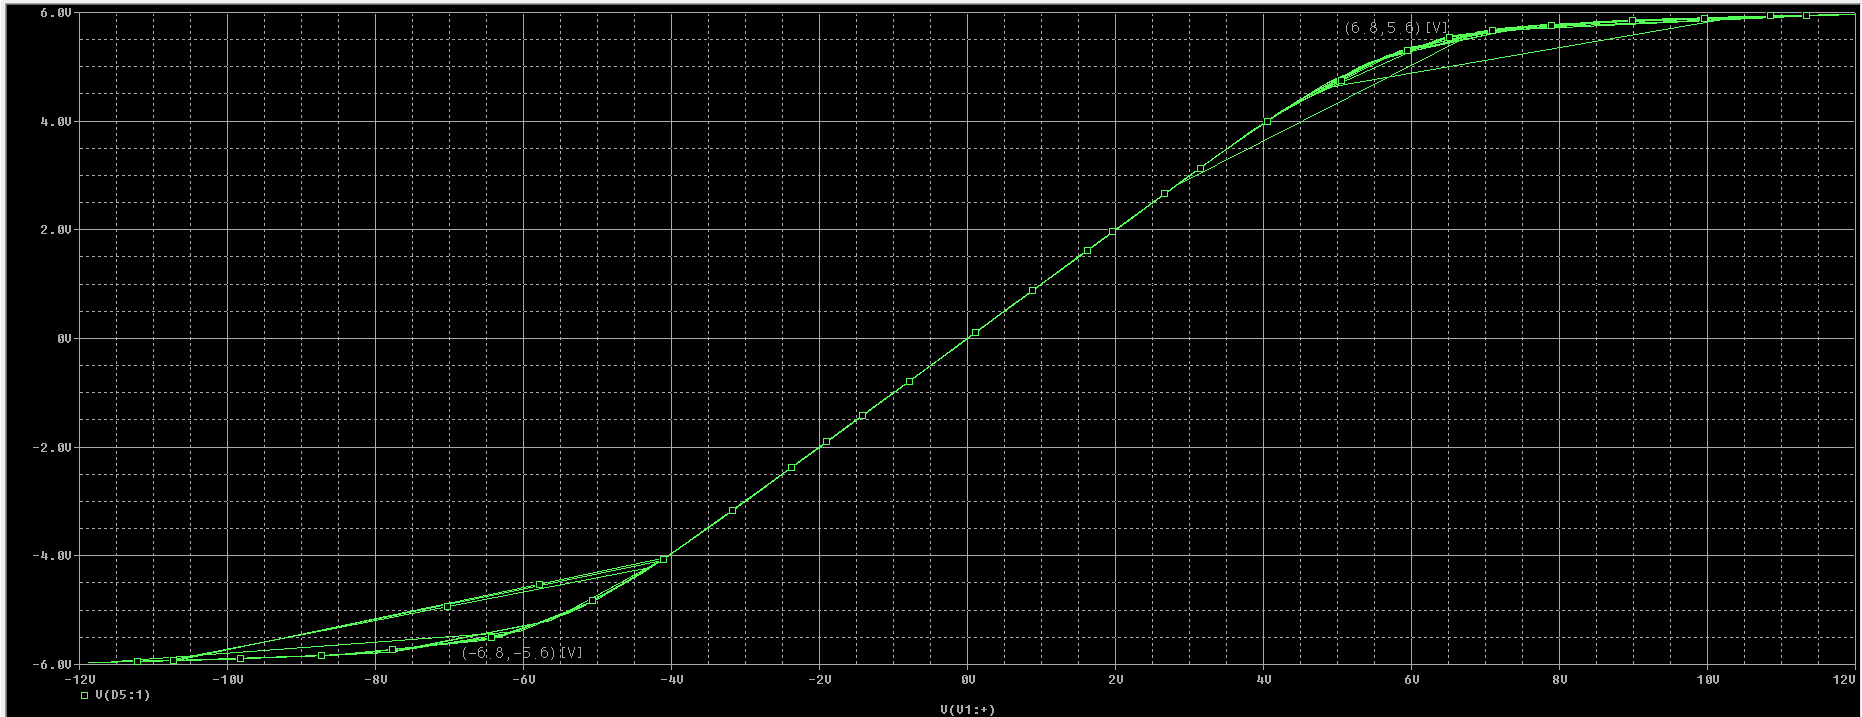
\includegraphics[width=.85\textwidth]{Figures/HW4-5e}
      \caption{Transfer Characteristics for $12[\si{\volt}]$ Amplitude Input}
      \label{fig:15}
    \end{figure}

    We may note that, for the $3[\si{\volt}]$ amplitude, the transfer characteristics are a perfect line, with a slope of 1. This is due to the fact that $\pm3[\si{\volt}]$ is within the permitted voltage range of the diodes; however, the $12[\si{\volt}]$ amplitude exceeds the $\pm6[\si{\volt}]$ input range. This causes the curve to become 'S' shaped, where it tapers off as the magnitudes approach $6[\si{\volt}]$. Furthermore, note that the knee values occur at the same points, indicating that, for diodes, only the magnitude, and not frequency, of the input make a difference.

\end{enumerate}

\end{document}

